% Editable standalone vector figure extracted from novogaia_spectra.tex.
% Source slide 16; figure 15; native embedded fonts.
% Compile with LuaLaTeX from this directory, or run ../export_figures.py.
\documentclass[tikz,border=0pt]{standalone}
% Shared editable preamble for standalone, Nature-style vector figures.
% Text remains embedded and searchable. This is a house-style target, not a
% claim of acceptance or of satisfying every journal's submission checklist.
\usepackage{fontspec}
\setmainfont{LiberationSans}[
  Path=../assets/,Extension=.ttf,
  UprightFont=*-Regular,BoldFont=*-Bold,ItalicFont=*-Italic,BoldItalicFont=*-BoldItalic]
\setsansfont{LiberationSans}[
  Path=../assets/,Extension=.ttf,
  UprightFont=*-Regular,BoldFont=*-Bold,ItalicFont=*-Italic,BoldItalicFont=*-BoldItalic]
\setmonofont{LiberationSans}[
  Path=../assets/,Extension=.ttf,
  UprightFont=*-Regular,BoldFont=*-Bold,ItalicFont=*-Italic,BoldItalicFont=*-BoldItalic]
\usepackage{unicode-math}
\setmathfont{Latin Modern Math}
\DeclareMathSizes{5.9}{6}{5}{5}
\DeclareMathSizes{6}{6}{5}{5}
\usepackage{tikz}
\usetikzlibrary{arrows.meta,calc,positioning,patterns,decorations.pathreplacing,matrix}
\usepackage{graphicx}
\usepackage{xcolor}
\pagecolor{white}
\definecolor{ink}{HTML}{202020}
\definecolor{paper}{HTML}{FFFFFF}
\definecolor{muted}{HTML}{494949}
\definecolor{line}{HTML}{808080}
\definecolor{soft}{HTML}{F0F0F0}
\hyphenpenalty=10000\exhyphenpenalty=10000
\newcommand{\figurefont}{\sffamily\fontsize{5.9}{7.4}\selectfont}
\newcommand{\figuremathfont}{\sffamily\fontsize{6}{7.5}\selectfont}
\newcommand{\brandmedium}{\bfseries}
\renewcommand{\normalsize}{\figurefont}
\renewcommand{\small}{\figurefont}
\renewcommand{\footnotesize}{\figurefont}
\renewcommand{\scriptsize}{\figurefont}
\renewcommand{\tiny}{\figurefont}
\renewcommand{\large}{\figurefont}
\renewcommand{\Large}{\figurefont}
\renewcommand{\LARGE}{\figurefont}
\renewcommand{\huge}{\figurefont}
\renewcommand{\Huge}{\figurefont}
\tikzset{
  every path/.style={line width=.55pt},
  every node/.style={font=\figurefont,text=ink},
  arr/.style={-{Latex[length=1.5mm,width=1mm]},line width=.55pt,draw=ink},
  thinarr/.style={-{Latex[length=1.3mm,width=.9mm]},line width=.55pt,draw=ink},
  box/.style={draw=ink,line width=.55pt,fill=white,minimum height=.85cm,align=center,inner sep=3pt},
  ghost/.style={draw=muted,dashed,fill=soft},
  tag/.style={font=\figurefont,text=muted},
  equ/.style={font=\figuremathfont},
  small/.style={font=\figurefont},
  body/.style={font=\figurefont},
  tinytext/.style={font=\figurefont}
}
\newcommand{\txt}[4]{\node[anchor=north west,align=left,text width=#3cm] at (#1,#2) {#4};}
\newcommand{\smalltxt}[4]{\node[anchor=north west,align=left,text width=#3cm,small] at (#1,#2) {#4};}
\newcommand{\eqn}[4][6]{\node[anchor=north west,font=\figuremathfont] at (#2,#3) {$\displaystyle #4$};}
\newcommand{\diagramblock}[5]{\node[box,minimum width=#3cm,text width=#3cm,minimum height=#4cm] at (#1,#2) {#5};}
% Scale coordinates, not text: all labels retain one final publication size.
\newcommand{\spectrum}[3]{\begin{scope}[shift={(#1,#2)}]
  \draw[muted] (0,0)--({3.6*#3},0);
  \draw[muted] (0,0)--(0,{1.9*#3});
  \foreach \x/\h in {.25/.18,.49/.46,.68/1.42,.87/.37,1.08/.74,1.31/.31,1.57/1.78,1.76/.46,1.96/.19,2.17/1.1,2.37/.57,2.57/.31,2.88/.76,3.21/.23,3.4/.38}{
    \draw[ink] ({\x*#3},0)--({\x*#3},{\h*#3});}
  \foreach \x in {.6,1.2,1.8,2.4,3.0}{\draw[ink] ({\x*#3},0)--+(0,{-.06*#3});}
  \foreach \y in {.45,.9,1.35,1.8}{\draw[ink] (0,{\y*#3})--+({-.06*#3},0);}
  \foreach \x/\lab in {0/0,1.8/45,3.6/90}{\node[anchor=north,font=\figurefont] at ({\x*#3},{-.08*#3}) {\lab};}
  \foreach \y/\lab in {0/0,.9/0.5,1.8/1.0}{\node[anchor=east,font=\figurefont] at ({-.08*#3},{\y*#3}) {\lab};}
  \node[anchor=north east,font=\figurefont] at ({3.6*#3},{-.45*#3}) {$m/z$ (Th)};
  \node[anchor=south west,font=\figurefont] at (0,{1.96*#3}) {Relative intensity (a.u.)};
\end{scope}}
\newcommand{\molecule}[3]{\begin{scope}[shift={(#1,#2)}]
  \draw[ink] (0,{#3})--({.866*#3},{.5*#3})--({.866*#3},{-.5*#3})--(0,{-#3})--({-.866*#3},{-.5*#3})--({-.866*#3},{.5*#3})--cycle;
  \draw[ink] ({.68*#3},{.4*#3})--({.68*#3},{-.4*#3});
  \draw[ink] ({-.7*#3},{-.44*#3})--({-.02*#3},{-.83*#3});
  \draw[ink] ({-.7*#3},{.44*#3})--({-.02*#3},{.83*#3});
  \draw[ink] (0,{#3})--(0,{1.55*#3});
  \node[font=\figurefont] at (0,{1.77*#3}) {OH};
\end{scope}}
\newcommand{\peaktokens}[3]{\foreach \i in {0,...,5}{\pgfmathsetmacro{\xx}{#1+\i*.36}\draw[fill=#3,draw=ink] (\xx,#2) rectangle +(.24,.6);}}
\newcommand{\E}{\mathbb E}
\newcommand{\R}{\mathbb R}
\newcommand{\sg}{\operatorname{stopgrad}}
\newcommand{\LN}{\operatorname{LN}}
\newcommand{\softmax}{\operatorname{softmax}}

\begin{document}
\figurefont
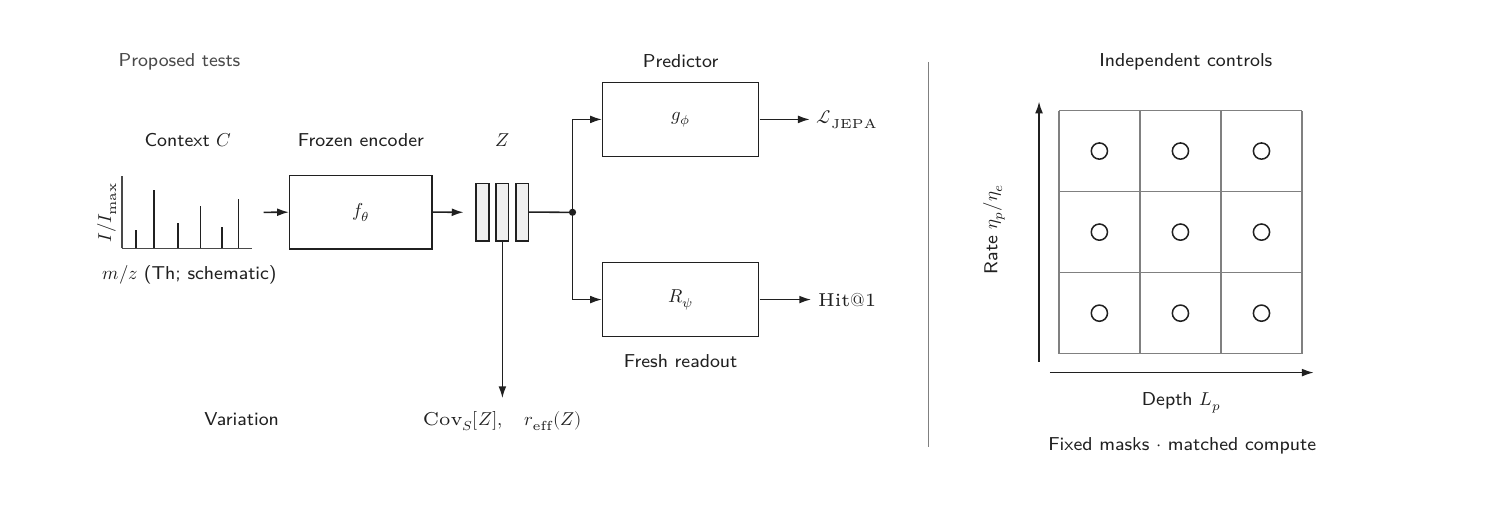
\begin{tikzpicture}[x=1cm,y=1cm,scale=1.14375,transform shape]
\node[anchor=base west,inner sep=0,tag] at (1.0,6.42) {Proposed tests};
% Context is an illustrative sparse spectrum; no hidden peaks or numeric claims.
\node[anchor=base,inner sep=0,small] at (1.77,5.53) {Context $C$};
\draw[muted,line width=.55pt] (1.05,4.40)--(2.49,4.40);
\draw[muted,line width=.55pt] (1.05,4.40)--(1.05,5.20);
\foreach \x/\h in {1.20/.20,1.40/.65,1.67/.28,1.92/.47,2.16/.24,2.34/.55}{\draw[ink,line width=.55pt] (\x,4.40)--+(0,\h);}
\node[anchor=base,inner sep=0,font=\figurefont] at (1.80,4.05) {$m/z$ (Th; schematic)};
\node[rotate=90,inner sep=0,font=\figurefont] at (.88,4.80) {$I/I_{\max}$};
\node[box,text width=1.30cm,inner xsep=4pt,minimum height=.82cm] (encoder) at (3.70,4.8) {$f_\theta$};
\node[anchor=base,inner sep=0,small] at (3.70,5.53) {Frozen encoder};
\draw[arr] (2.62,4.80)--(encoder.west);
% A row of coordinate tiles represents the encoder output.
\foreach \x in {4.98,5.20,5.42}{\draw[draw=ink,fill=soft,line width=.55pt] (\x,4.48) rectangle +(.14,.64);}
\node[anchor=base,inner sep=0,small] at (5.27,5.53) {$Z$};
\draw[arr] (encoder.east)--(4.84,4.80);
\coordinate (latentright) at (5.56,4.80);
\coordinate (latentbottom) at (5.27,4.48);
\node[box,text width=1.45cm,inner xsep=4pt,minimum height=.82cm] (predictor) at (7.25,5.83) {$g_\phi$};
\node[small] at (7.25,6.48) {Predictor};
\node[box,text width=1.45cm,inner xsep=4pt,minimum height=.82cm] (readout) at (7.25,3.83) {$R_\psi$};
\node[small] at (7.25,3.15) {Fresh readout};
\draw[ink,line width=.55pt] (latentright)--(6.05,4.80);
\fill[ink] (6.05,4.80) circle (.04);
\draw[arr] (6.05,4.80)|-(predictor.west);
\draw[arr] (6.05,4.80)|-(readout.west);
\node[font=\figurefont,inner sep=2pt] (loss) at (9.10,5.83) {$\mathcal L_{\rm JEPA}$};
\node[font=\figurefont,inner sep=2pt] (hit) at (9.10,3.83) {$\mathrm{Hit@1}$};
\draw[arr] (predictor.east)--(loss.west);
\draw[arr] (readout.east)--(hit.west);
\node[anchor=base,inner sep=0] (variation) at (5.27,2.43) {$\operatorname{Cov}_{S}[Z],\quad r_{\rm eff}(Z)$};
\node[anchor=base east,inner sep=0,small] at (2.80,2.43) {Variation};
\draw[arr] (latentbottom)--([yshift=4pt]variation.north);
\draw[line,line width=.55pt] (10.0,6.47)--(10.0,2.19);
\node[small] at (12.86,6.47) {Independent controls};
\foreach \x in {11.45,12.35,13.25,14.15}{\draw[line,line width=.55pt] (\x,3.23)--(\x,5.93);}
\foreach \y in {3.23,4.13,5.03,5.93}{\draw[line,line width=.55pt] (11.45,\y)--(14.15,\y);}
\foreach \x in {11.90,12.80,13.70}{\foreach \y in {3.68,4.58,5.48}{\draw[ink,line width=.55pt,fill=paper] (\x,\y) circle (.09);}}
\draw[arr] (11.35,3.02)--(14.28,3.02);
\draw[arr] (11.23,3.14)--(11.23,6.03);
\node[anchor=base,inner sep=0,small] at (12.81,2.65) {Depth $L_p$};
\node[small,rotate=90] at (10.73,4.61) {Rate $\eta_p/\eta_e$};
\node[anchor=base,inner sep=0,small] at (12.82,2.16) {Fixed masks $\cdot$ matched compute};
% Fixed canvas: 183 x 60.046875 mm. No clipping: overflow is audited.
\pgfresetboundingbox
\path[use as bounding box] (0,1.6) rectangle (16,6.85);
\end{tikzpicture}
\end{document}
